\documentclass{article}

% tight measures:
% \usepackage[margin=0mm, paperwidth=56mm, paperheight=42mm]{geometry}
% loose measures:
\usepackage[margin=2mm, paperwidth=60mm, paperheight=45.5mm]{geometry}

\usepackage{amsmath}
\usepackage{tikz}
\usetikzlibrary{bayesnet}
\usepackage{bm}
\providecommand{\mathbold}[1]{\bm{#1}}
\newcommand{\vct}[1]{\mathbold{#1}}

\begin{document}
\thispagestyle{empty}

\begin{center}
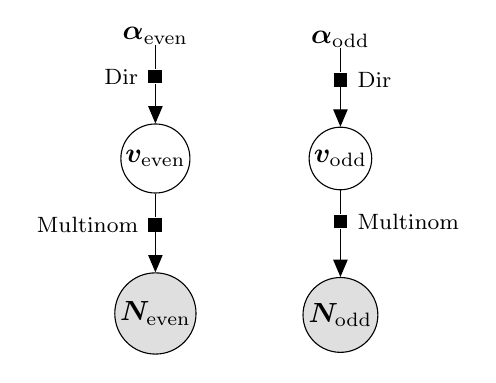
\begin{tikzpicture}
   \node[latent] (veven) {$\vct{v}_{\text{even}}$} ;
   \node[latent, right=1.5 of veven] (vodd) {$\vct{v}_{\text{odd}}$} ;
   \node[const, above= of veven] (alpeven) {$\vct{\alpha}_{\text{even}}$} ;
   \node[const, above= of vodd] (alpodd) {$\vct{\alpha}_{\text{odd}}$} ;
   \node[obs, below=1 of veven] (Neven) {$\vct{N}_{\text{even}}$} ;
   \node[obs, below=1.1 of vodd] (Nodd) {$\vct{N}_{\text{odd}}$} ;
   \factor[above=.5 of veven] {alpeven-veven} {left:Dir} {alpeven} {veven} ;
   \factor[above=.5 of vodd] {alpodd-vodd} {right:Dir} {alpodd} {vodd} ;
   \factor[below=.3 of veven] {veven-Neven} {left:Multinom} {veven} {Neven} ;
   \factor[below=.3 of vodd] {vodd-Nodd} {right:Multinom} {vodd} {Nodd} ;
\end{tikzpicture}
\end{center}

\end{document}











